
In this chapter, I provide experimental evidence for the claims made
in earlier chapters. I will begin by describing my experimental setup, and
outline the methods used for the subsequent tests. Three sections follow, each
examining a different performance aspect. The first of these sections aims to
replicate and extend the results of Yoneki et al\cite{crackle} in
optimal a prefetching strategy for Grapht. The next section examines the
performance of certain queries across the three database engines under
consideration: PostgreSQL, Grapht and Neo4J. This allows me both to confirm
the premise motivating the development of Grapht -- that there exist large
performance gaps in both directions between PostgreSQL and Neo4J -- and to show
that the addition of an intermediate hybrid query processor can help to bridge
this gap and improve average overall performance. Finally, the last section
includes a qualitative examination of the expressiveness of the
three query systems, both in terms in terms of the declarative query language
presented, and in terms the direct API offered where one is available.

\section{Test Framework}

Before undertaking any tests, an experimental hypothesis was chosen to direct
the direction of my investigations. These hypotheses are outlined in the
appropriate sections. To obtain a measure for query performance, a Scala
benchmarking program was written, which recorded the start and end time of
operations and used these to calculate the average execution time for each operation.
Each  query was performed ten times, with the fastest and slowest results
discarded as outliers. Unless otherwise stated, 100 queries of approximately
the same size were randomly chosen for each test, to prevent the
particularities of any single query from impacting the overall results. For PostgreSQL and Neo4J, a cache-warming query was performed before
each test by iterating through every vertex in the graph. This was not
performed for Grapht, since such a cache-warming query would cause the
prefetcher to load much of the graph into memory, making  the presence of the
prefetcher redundant by the time the query is performed. This disparity is
tolerable, since we nonetheless will see  a conservative estimate for Grapht's
performance with respect to our performance hypotheses.

The same dataset was pre-loaded into both PostgreSQL and Neo4J, consisting of
a DIMACS dataset representing the U.S. road network\cite{dimacs}. This graph
contained 264,346 vertices and 733,846 edges. Both edges and vertices were then
augmented with a ``\texttt{payload}'' attribute calculated as the MD5 hash of the
entity ID. This was done to ensure that the database contained more than
simple topological information, as is likely to be the case for many practical
applications of graph databases. In PostgreSQL, the graph was defined by two
relations, as shown in Table~\ref{ta:postgresschema}. In Neo4J, the graph was
defined according to the standard graph format, with an index created on
vertex IDs, and attributes added to vertices and edges as entity
\textit{properties}.

All experiments were carried out using Ubuntu 16.04 running on a 3.4 GHz, 64-bit 4-core
Intel Core i7 processor (2nd generation), with 8 GB of RAM. JVM v1.8 was used,
with the maximum and minimum heap size set to 1024MB by default, to avoid
wasting time trying to acquire more memory from the system. The JVM has global
pauses for garbage collection, so a manual garbage collection was requested
before each test, to try and ensure that any pauses were at fault of the
current test itself. Note that in figures presented in the following sections, a logarithmic scale has been used for clarity, since there are often
performance differences of several orders of magnitude between the systems.


\section{Prefetcher Performance}
\label{sec:prefetcher_performance}

The first task was to select a prefetching strategy to use in Grapht. For this
evaluation, I examined the prefetchers described in section~\ref{impl:graph}.
In evaluating prefetcher performance, the initial expectation was to find that
the peak performance would come from prefetching with large blocks rather than
using a lookahead strategy -- as reported by Yoneki et al. In addition, where
the original CTE prefetcher suffered as lookahead depth increased, I expected
to find that my iterative lookahead prefetcher would perform better by
performing cheaper queries at large depths.

To test the effects of changing prefetching strategies, I measured the execution time for
an A* search using each prefetcher. I consider here separately
five different query lengths, in order to see whether prefetching strategies
were particularly good or bad when examining larger portions of the graph.
Paths consisting of 20, 40, 60, 80 and 100 hops were each considered. Twenty
queries were selected for each path length by randomly selecting start and end
points within a graph neighbourhood, and performing a shortest-path
calculation to select vertices for which the shortest path had the desired length. The size of the
subgraph explored by the A* algorithm for each of these paths varied largely
by query, but was always 80-100 times the length of the path, such that subgraphs
containing up to 12,000 vertices were examined.

\begin{figure}[htbp]
	\centering
	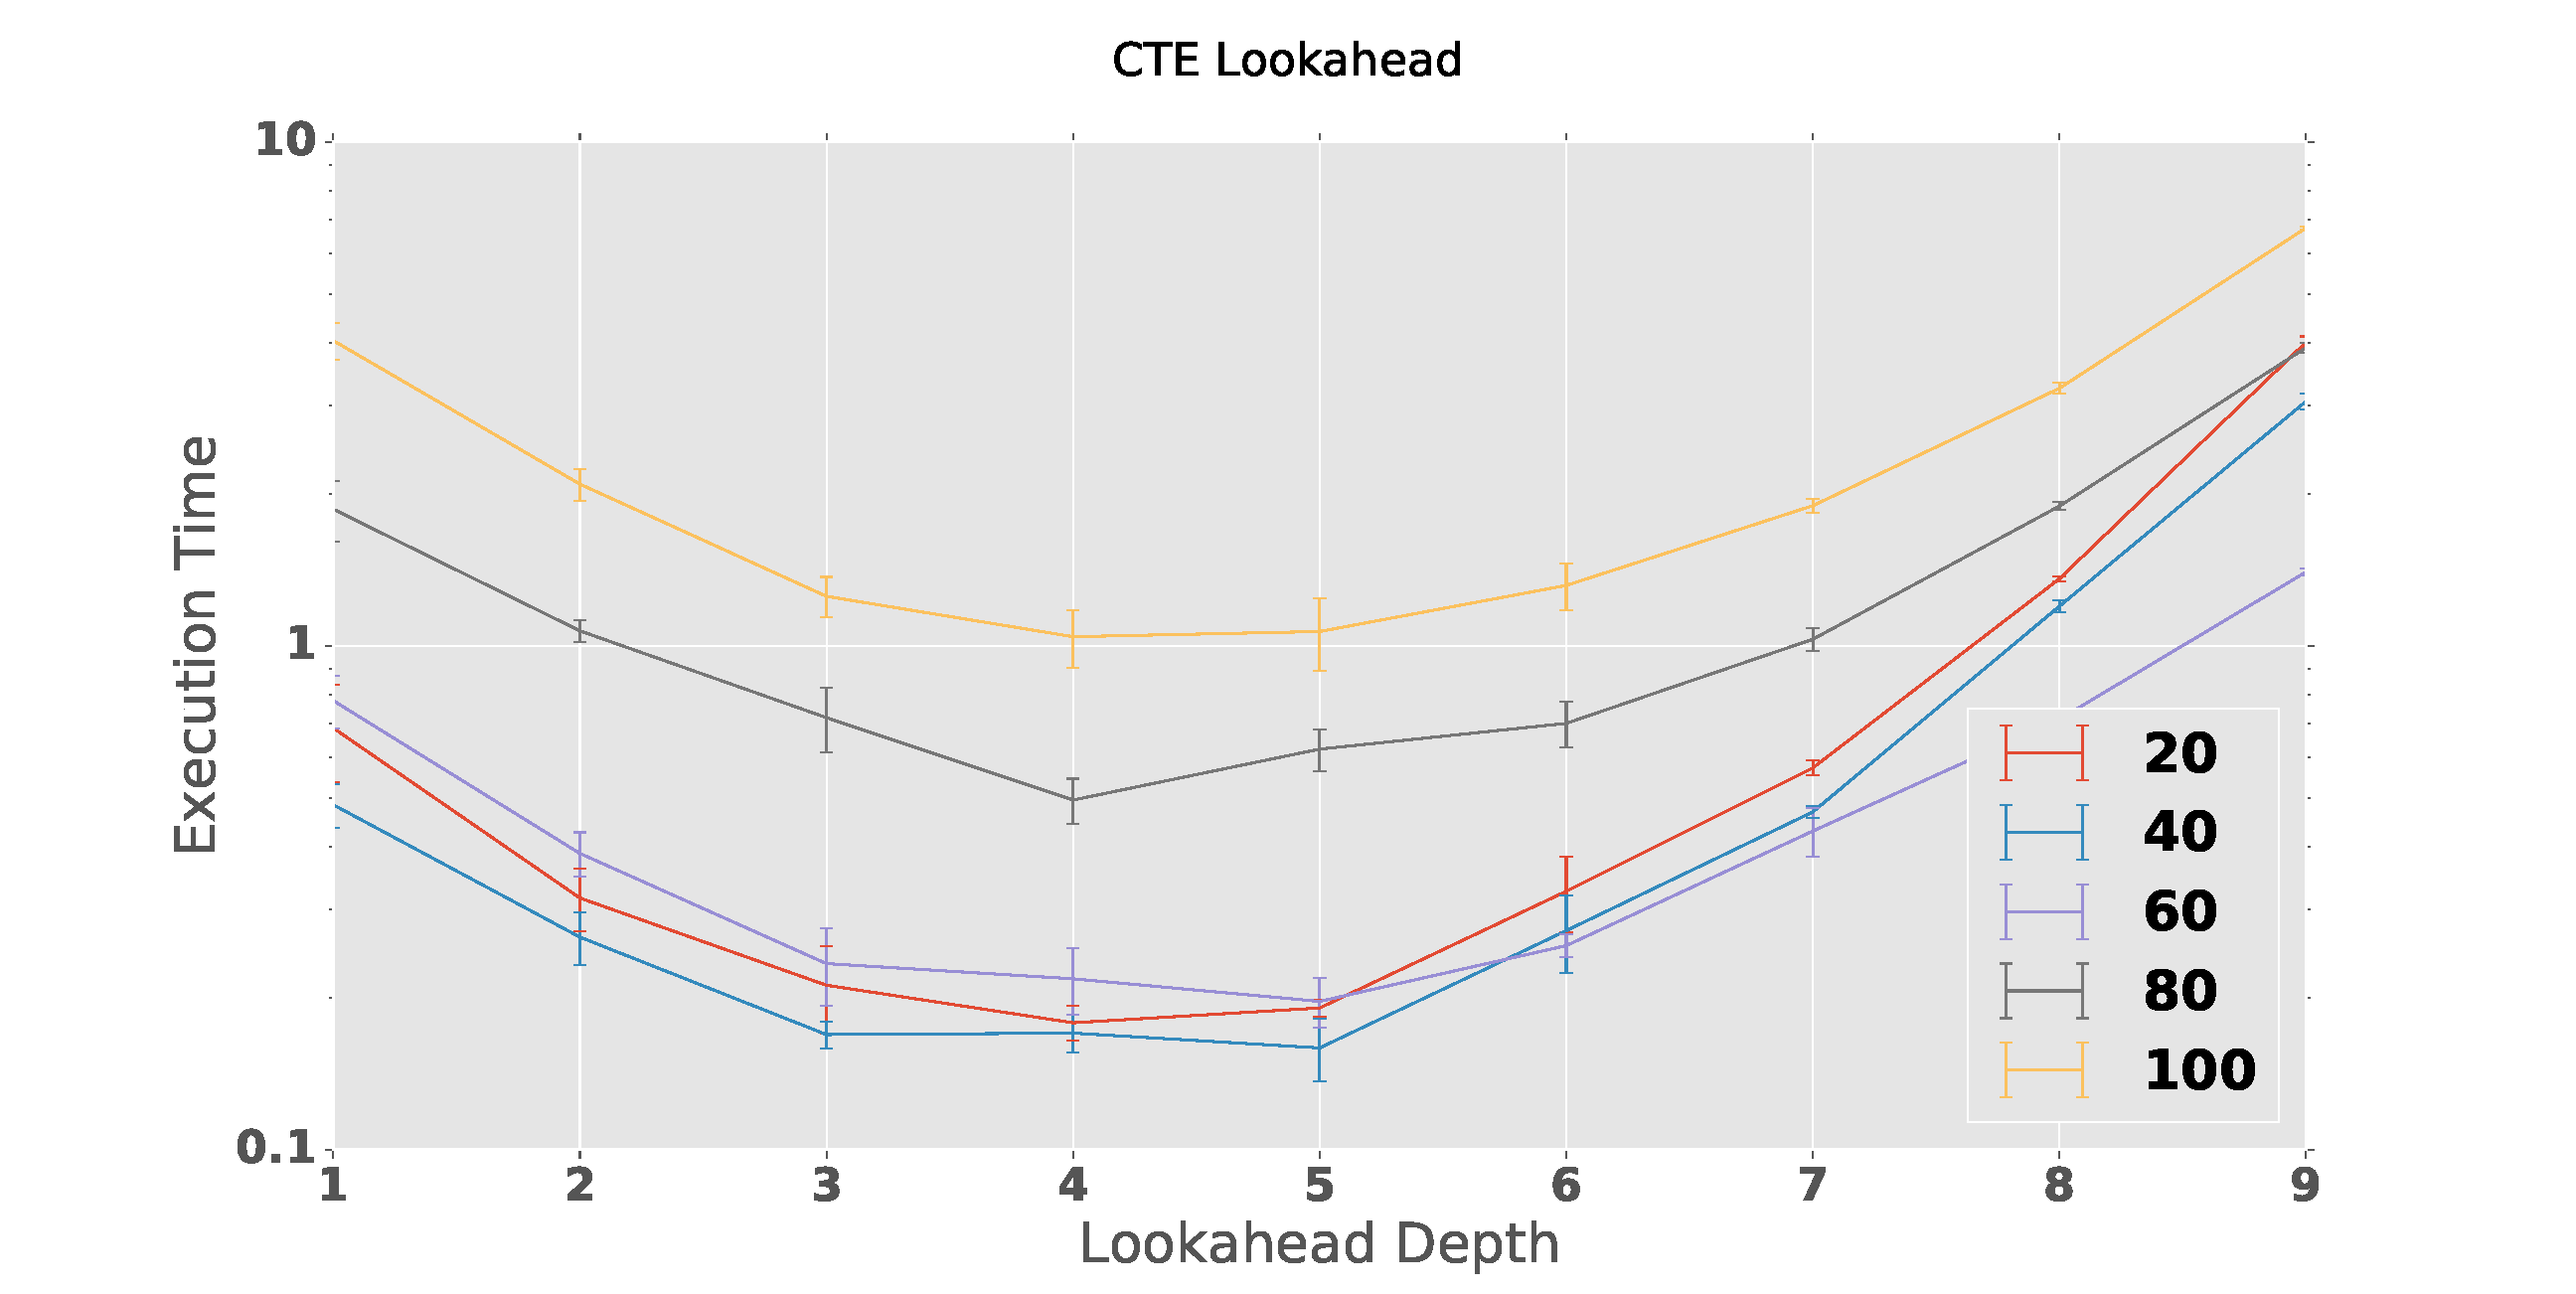
\includegraphics[width=0.95\textwidth]{figs/prefetch-CTE.eps}
	\caption{Average Execution time for A* search of different path lengths using a CTE lookahead prefetcher}
	\label{fig:prefetch-CTE}
\end{figure}
\begin{figure}[htbp]
	\centering
	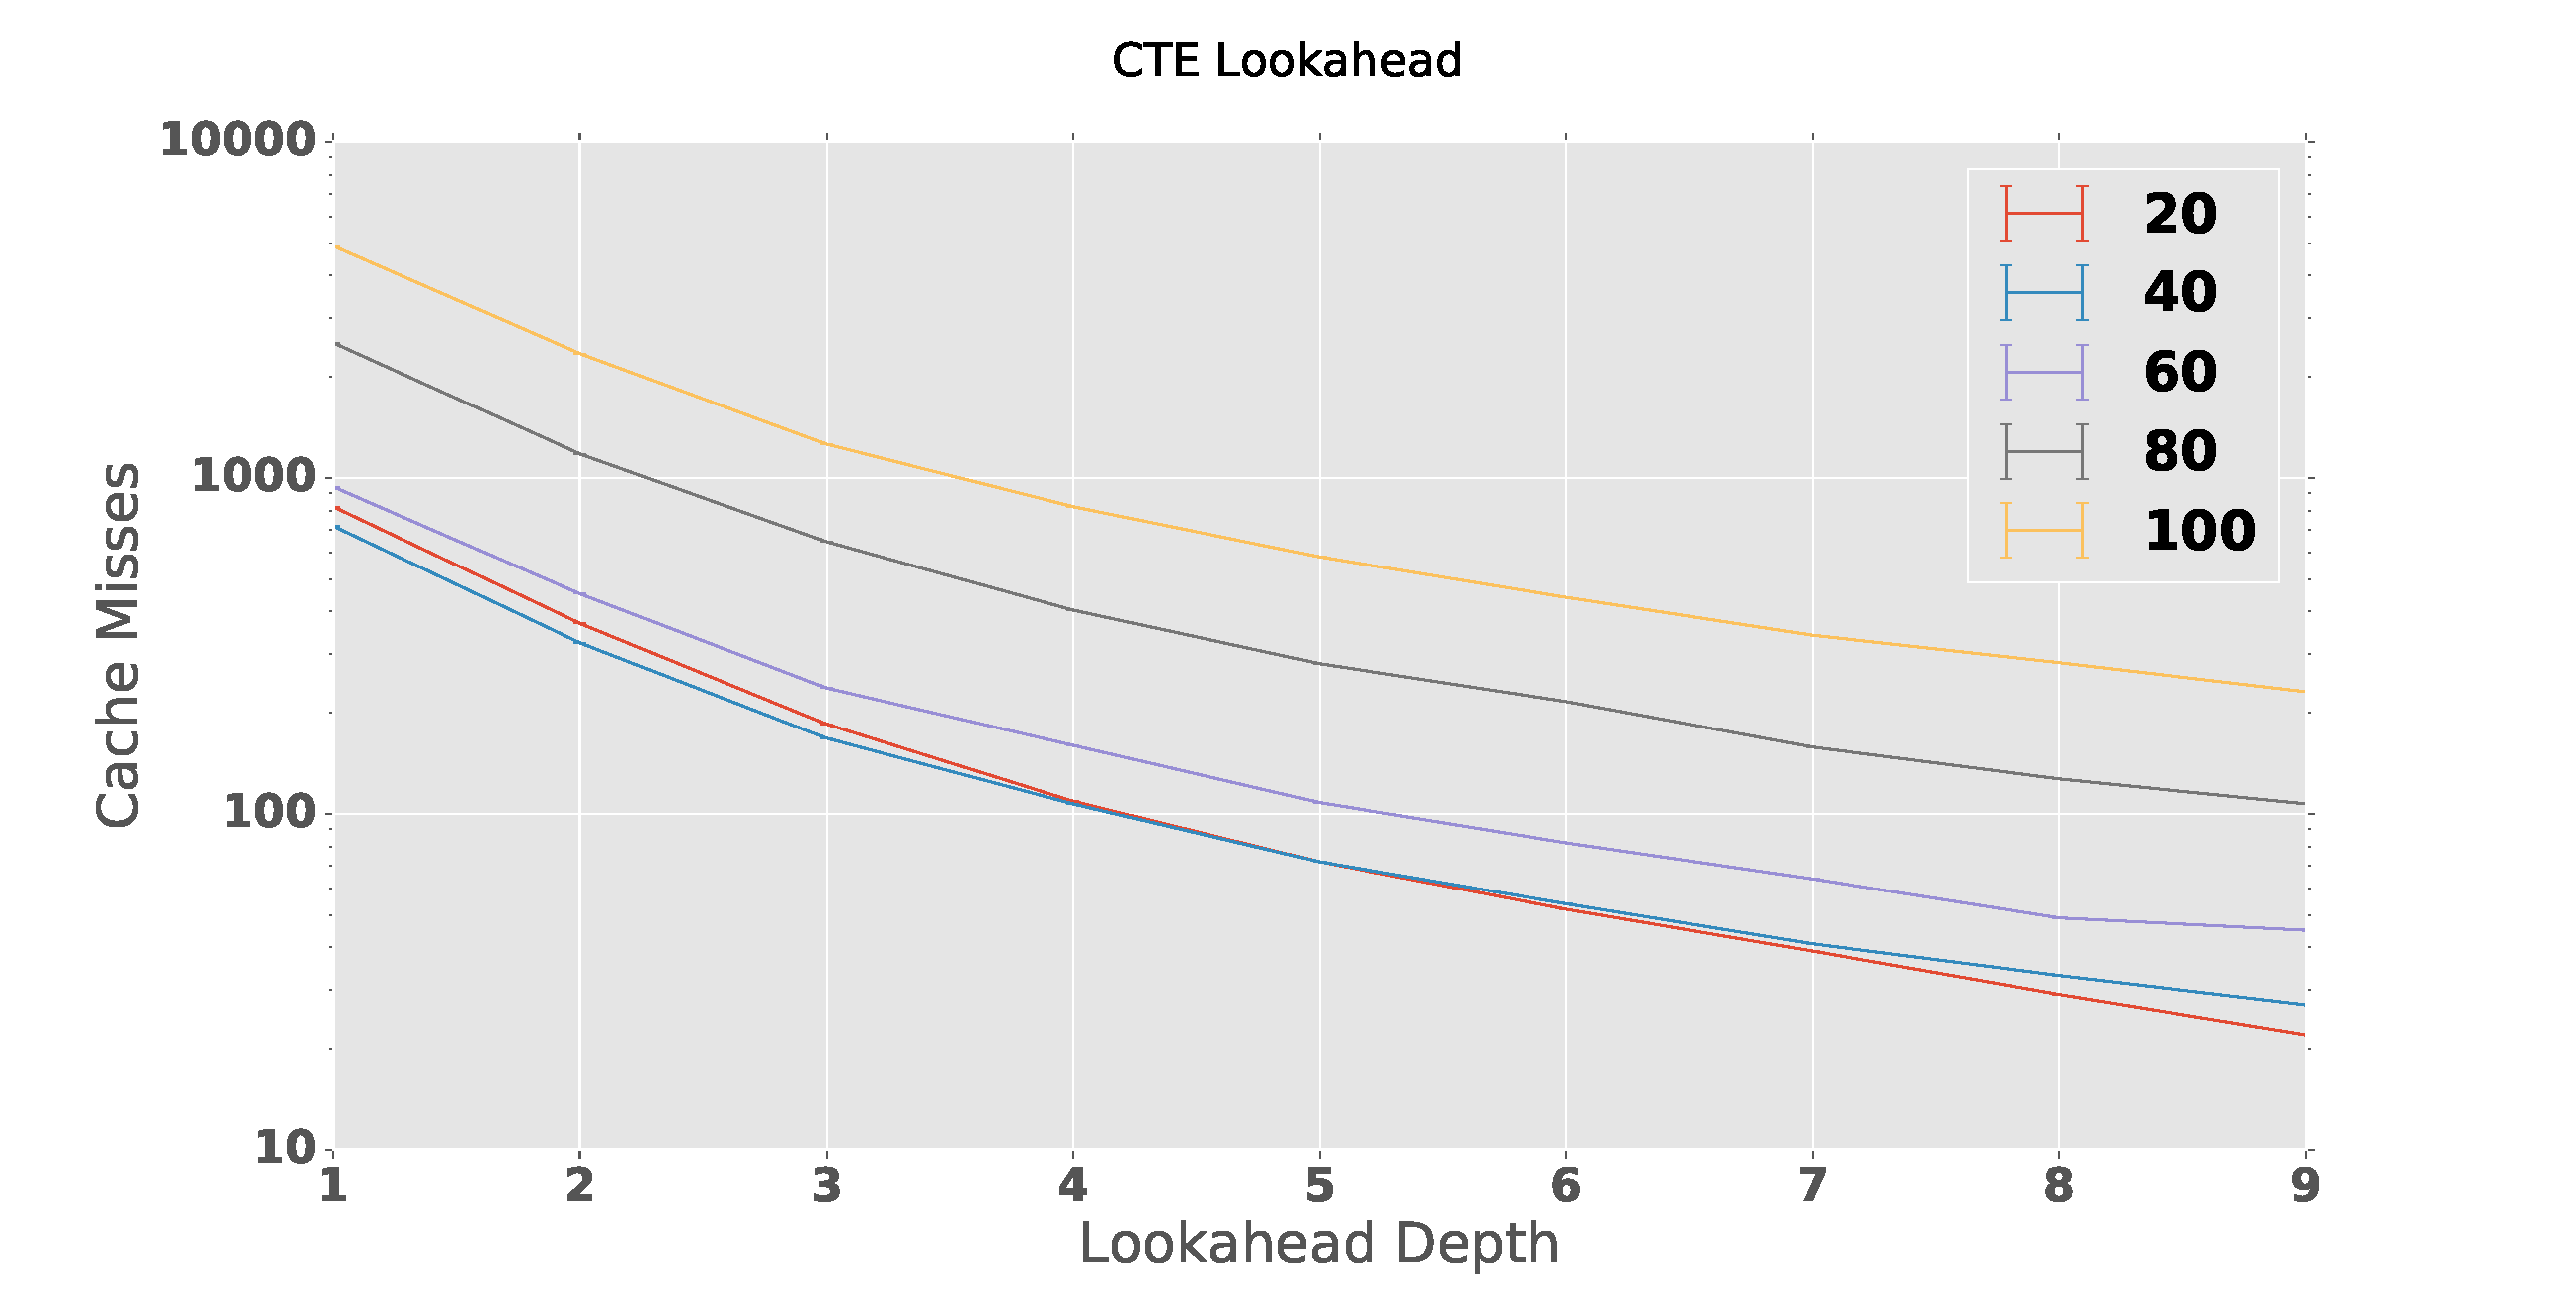
\includegraphics[width=0.95\textwidth]{figs/prefetch-misses-CTE.eps}
	\caption{Graph miss rate for A* search of different path lengths using a CTE lookahead prefetcher}
	\label{fig:prefetch-miss-CTE}
\end{figure}
\begin{figure}[htbp]
	\centering
	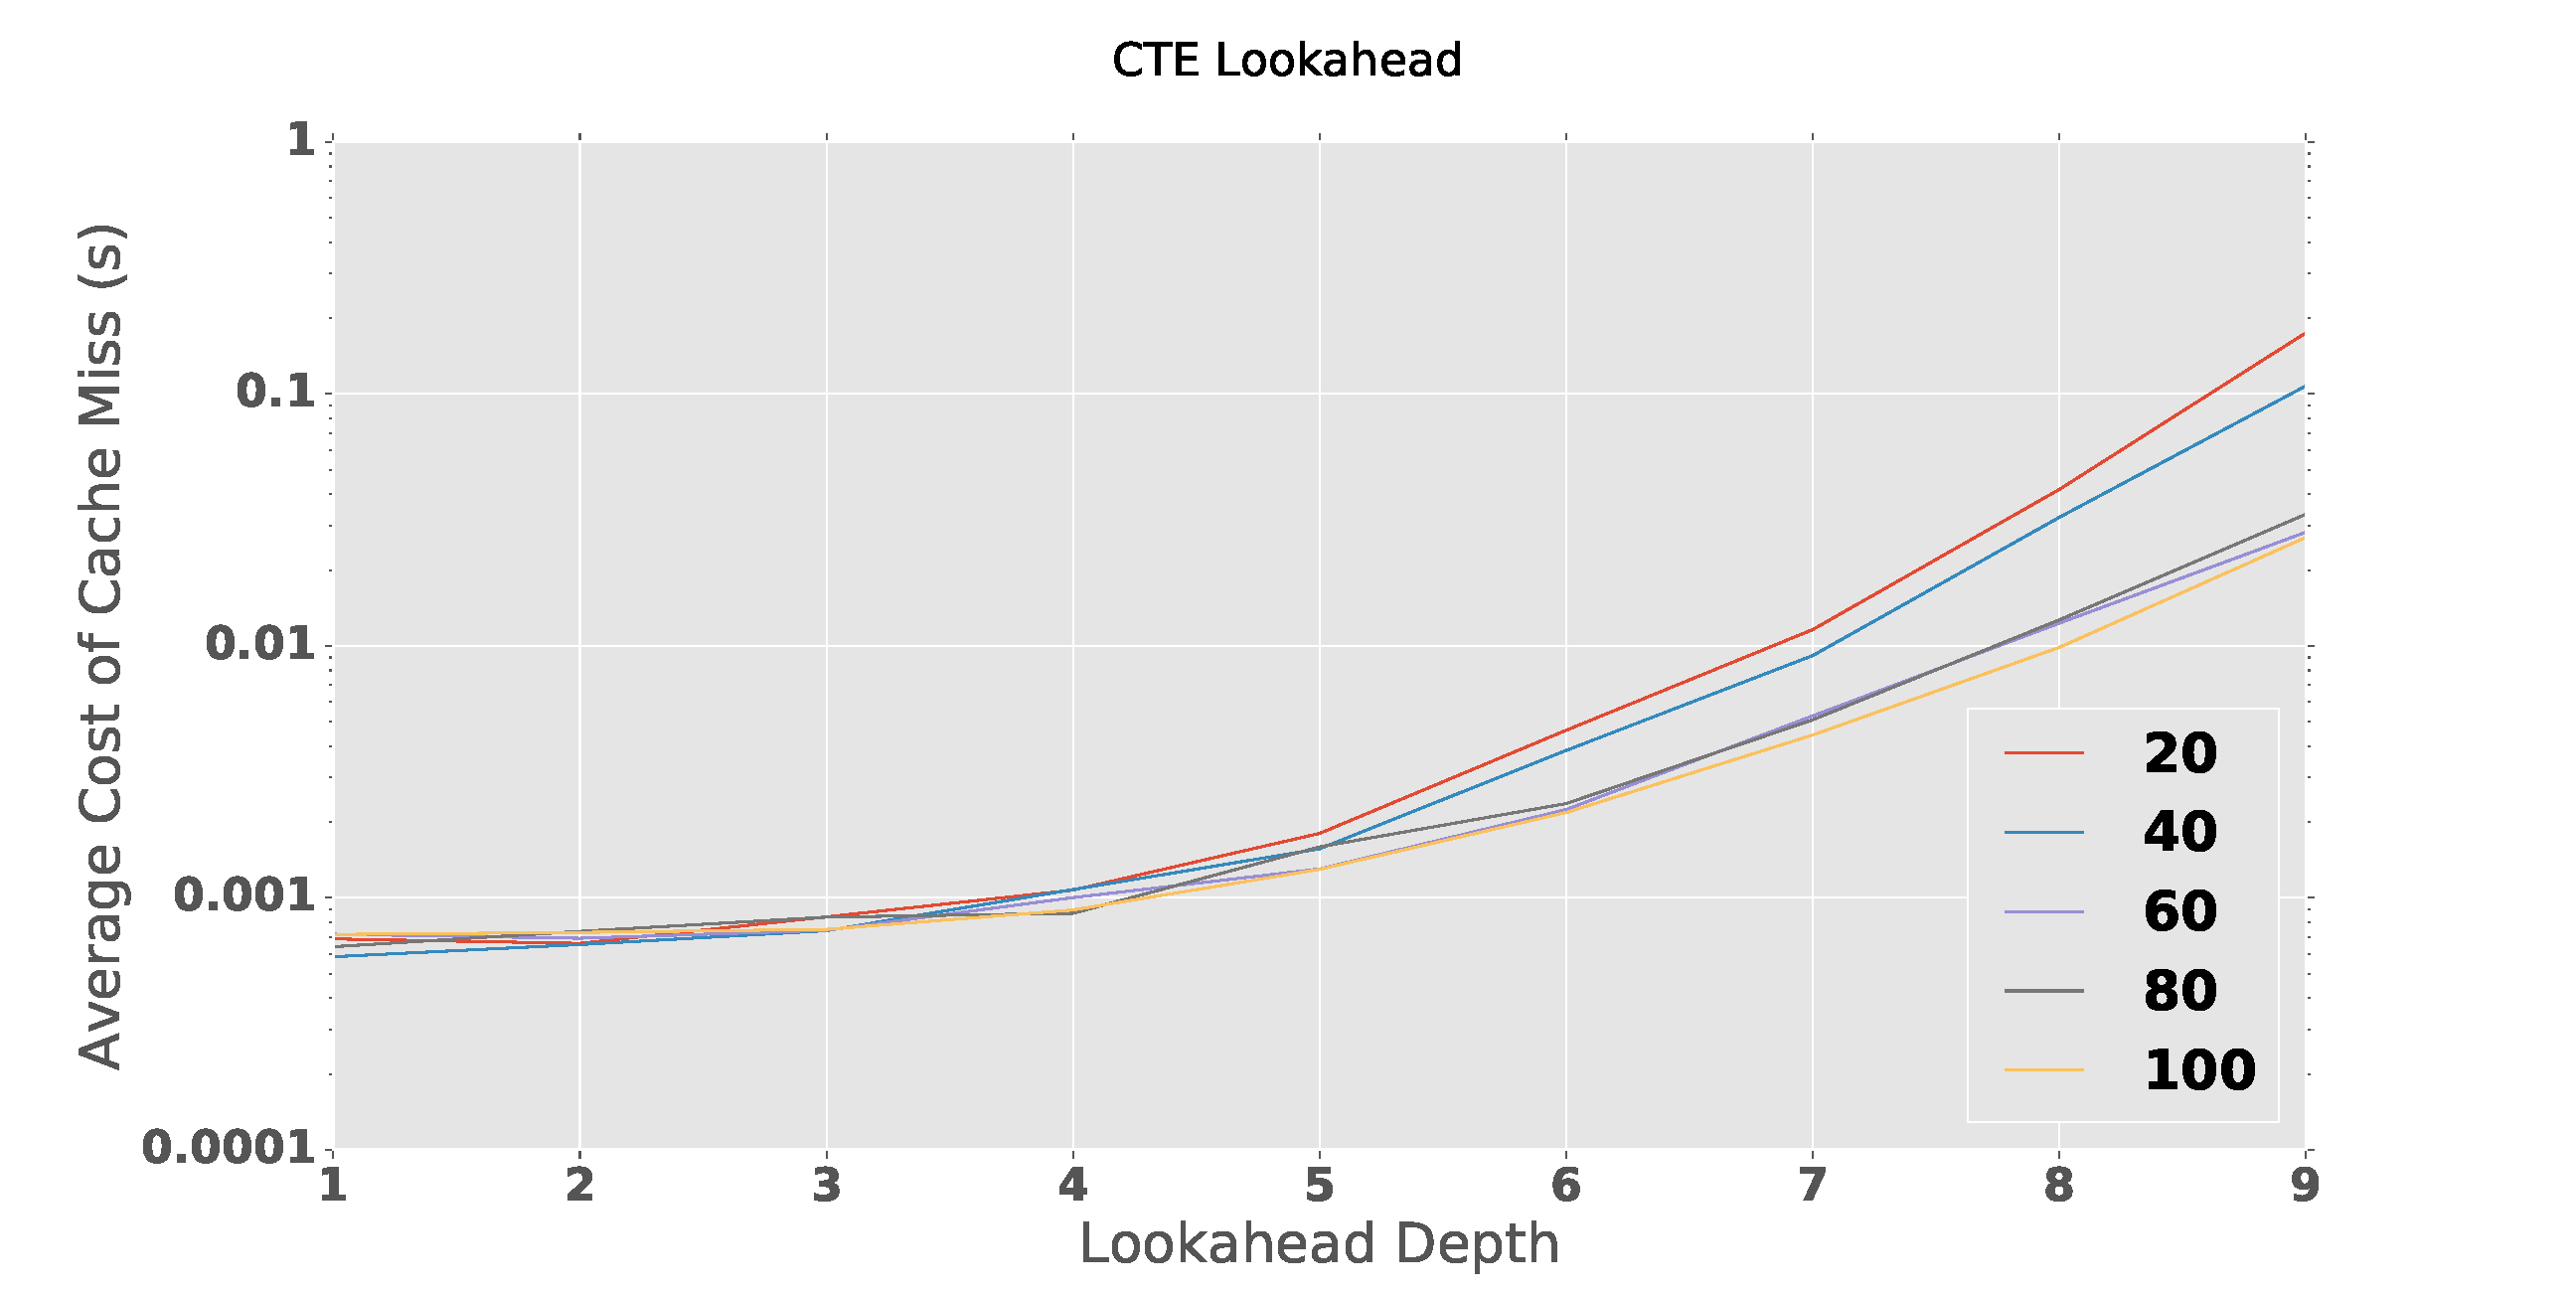
\includegraphics[width=0.95\textwidth]{figs/prefetch-dbcost-CTE.eps}
	\caption{Average cost of store miss for A* search of different path lengths using a CTE lookahead prefetcher}
	\label{fig:prefetch-dbcost-CTE}
\end{figure}

Figure~\ref{fig:prefetch-CTE} shows an analysis of the effect of changing the
depth of the CTE lookahead prefetcher. As expected, we see that for all path
lengths performance initially improves as we increase path length, until a
lookahead depth of around 4 to 5. At this point, execution time begins to
increase again. We can gain a better causal understanding of this behaviour by examining  the number of vertices needing to be fetched from the
database for each query (the store \textit{miss rate}). We see from
Figure~\ref{fig:prefetch-miss-CTE} that the miss rate decreases exponentially
as lookahead depth increases. This is expected since more vertices are fetched
with each miss. The overall execution time thus initially decreases with
depth. In contrast, the average cost of each store miss increases more than
exponentially (Figure~\ref{fig:prefetch-dbcost-CTE}). This cost quickly
overcomes the benefit from the reduced number of graph misses, and becomes the
dominating factor as lookahead depth increases.

\begin{figure}[htbp]
	\centering
	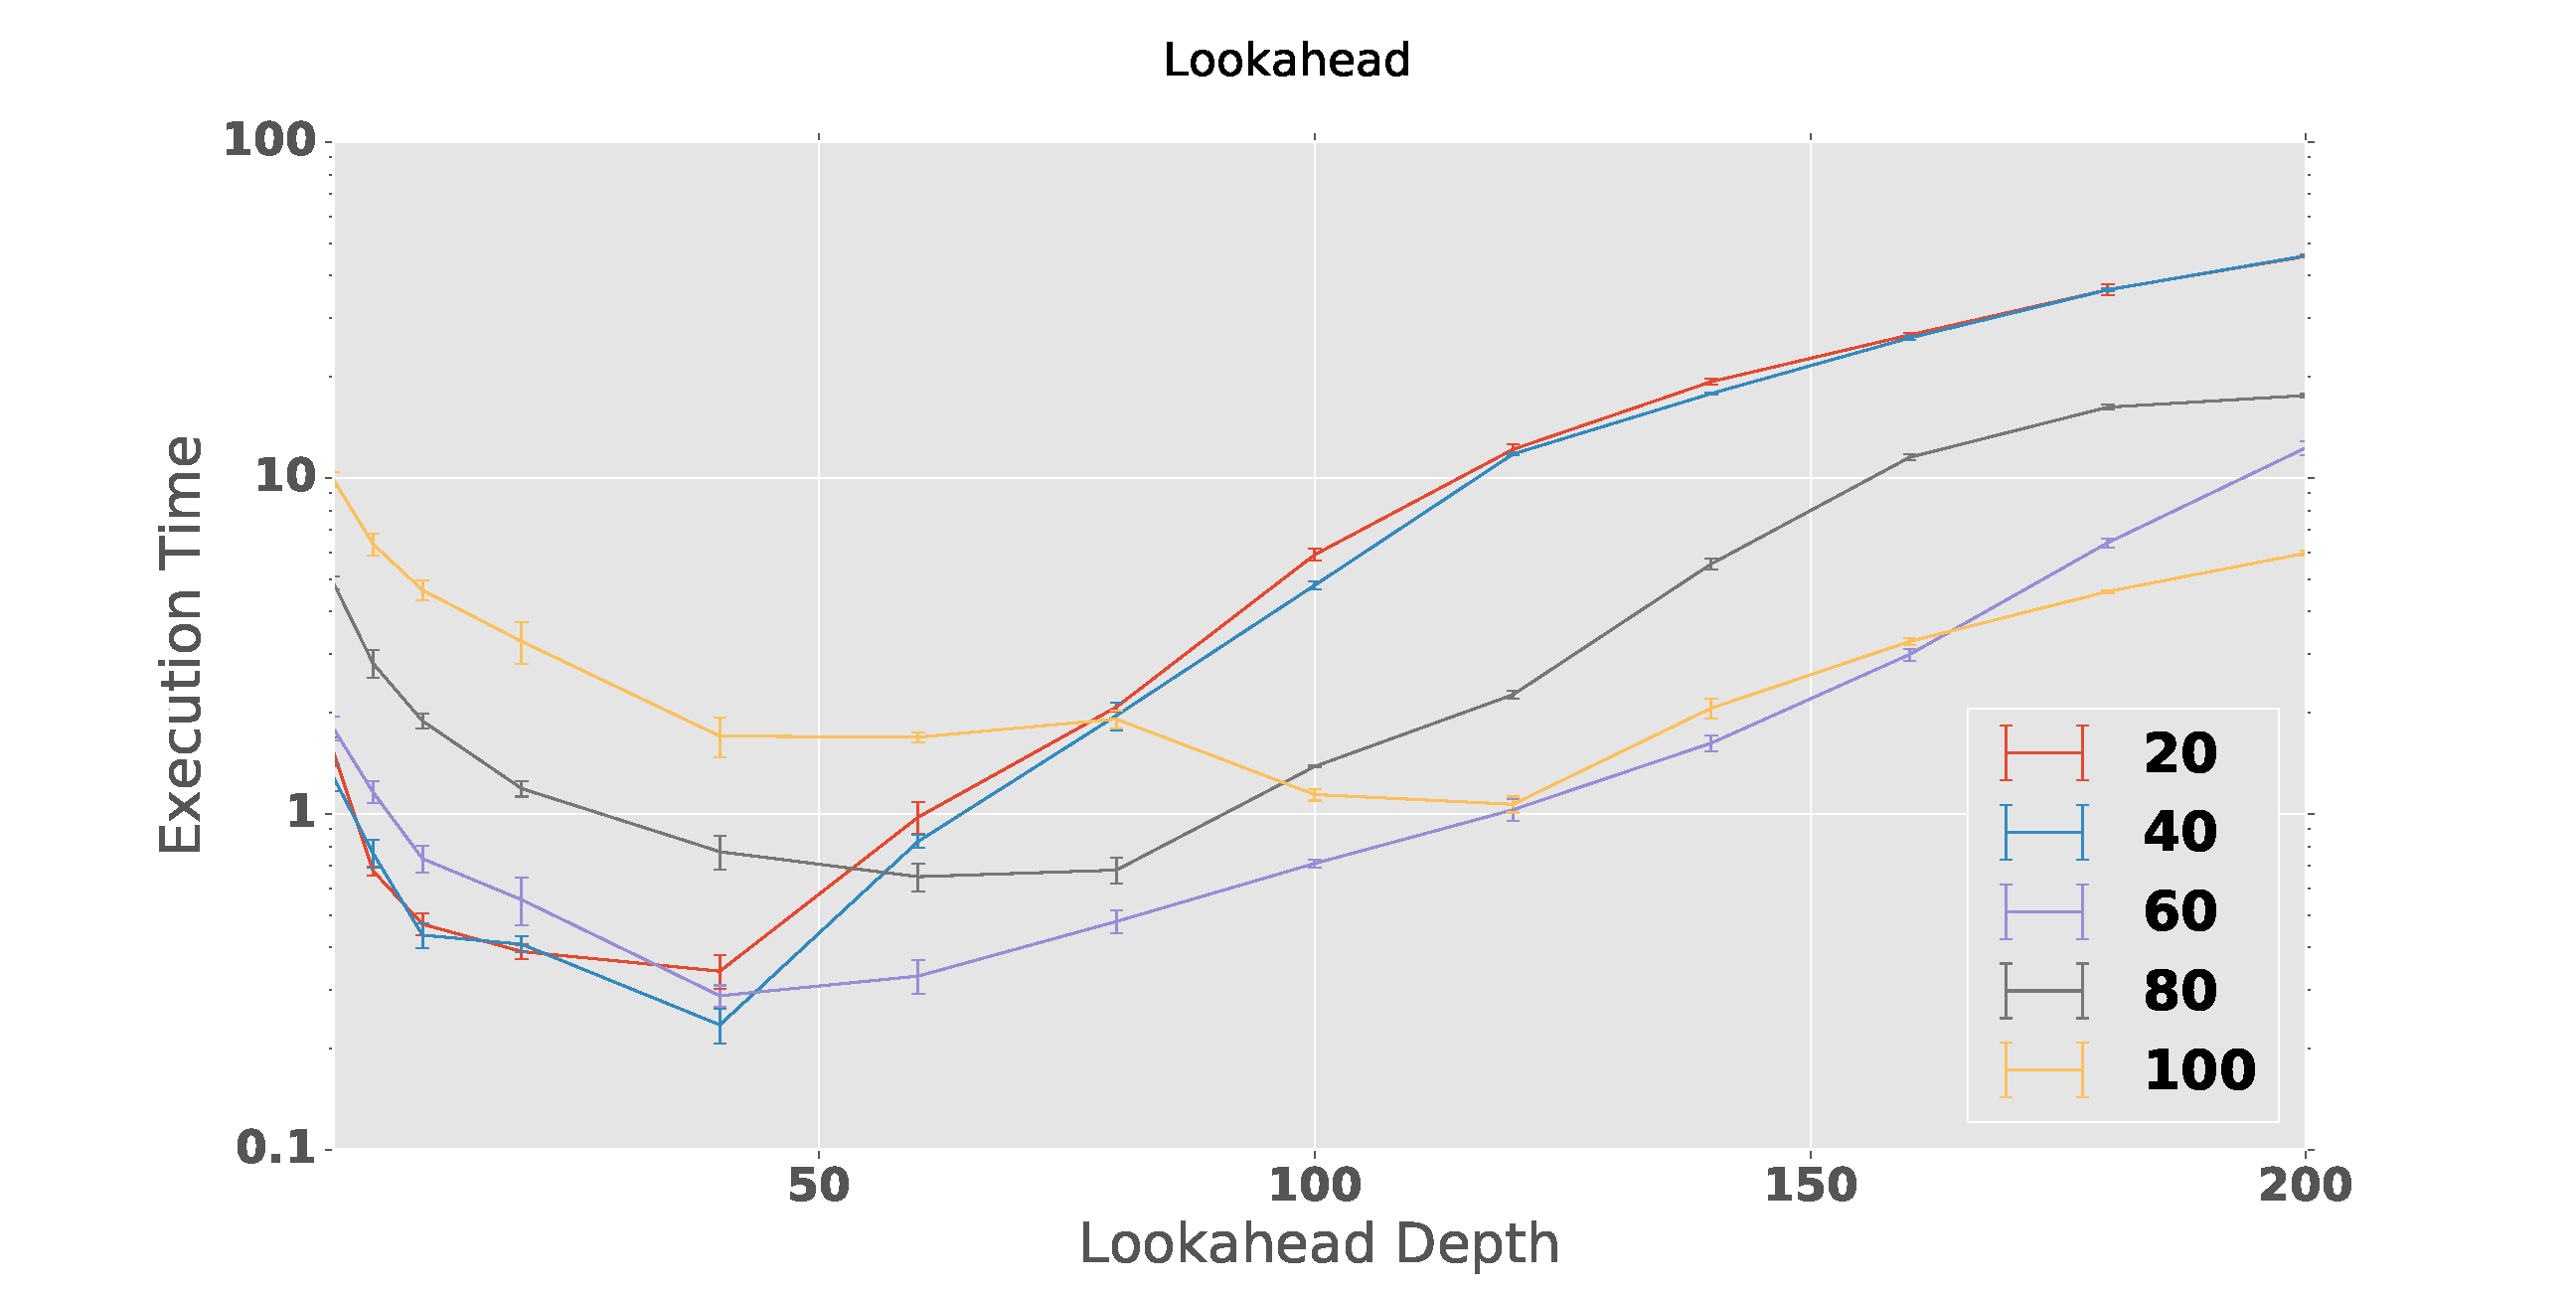
\includegraphics[width=0.95\textwidth]{figs/prefetch-itr.eps}
	\caption{Average Execution time for A* search of different path lengths using an iterative lookahead prefetcher}
	\label{fig:prefetch-lookahead}
\end{figure}
\begin{figure}[htbp]
	\centering
	\includegraphics[width=0.95\textwidth]{figs/prefetch-misses-itr.eps}
	\caption{Graph miss rate for A* search of different path lengths using an iterative lookahead prefetcher}
	\label{fig:prefetch-miss-lookahead}
\end{figure}
\begin{figure}[htbp]
	\centering
	\includegraphics[width=0.95\textwidth]{figs/prefetch-dbcost-itr.eps}
	\caption{Average cost of store miss for A* search of different path lengths using an iterative lookahead prefetcher}
	\label{fig:prefetch-dbcost-lookahead}
\end{figure}

For the iterative lookahead strategy, we see that the average cost of each
graph miss (Figure~\ref{fig:prefetch-dbcost-lookahead}) is initially higher
than for the CTE strategy. This is due to the fact that several queries are
performed at each iteration instead of a single more complex query. However the
average cost using the iterative approach grows far more slowly with lookahead
depth, allowing lookahead depths around five times larger than the CTE
approach to be used before performance starts to degrade. This larger
lookahead depth in turn causes a much lower store miss rate. Indeed, in all of
the examined queries, the lookahead depth was allowed to exceed the path size,
meaning that the store miss rate effectively settled at 1 (when only the
source vertex misses). The effect of these two factors on overall query
time is that the total time taken fetching vertices from the database
decreases steadily as the store miss rate decreases. As soon as the graph miss
rate reaches 1, however, the overall time taken increases with lookahead
depth. This happens because additional iterations only fetch vertices which will not be used, 
since they did not need fetching at lower lookahead depths. Although the peak performance of this approach is
similar to the CTE lookahead strategy for A* search, the overall performance
characteristics are quite different. It seems likely that the vastly increased
lookahead depth would improve performance for other types of queries where the graph miss
rate is never allowed to reach 1.

\begin{figure}[htbp]
	\centering
	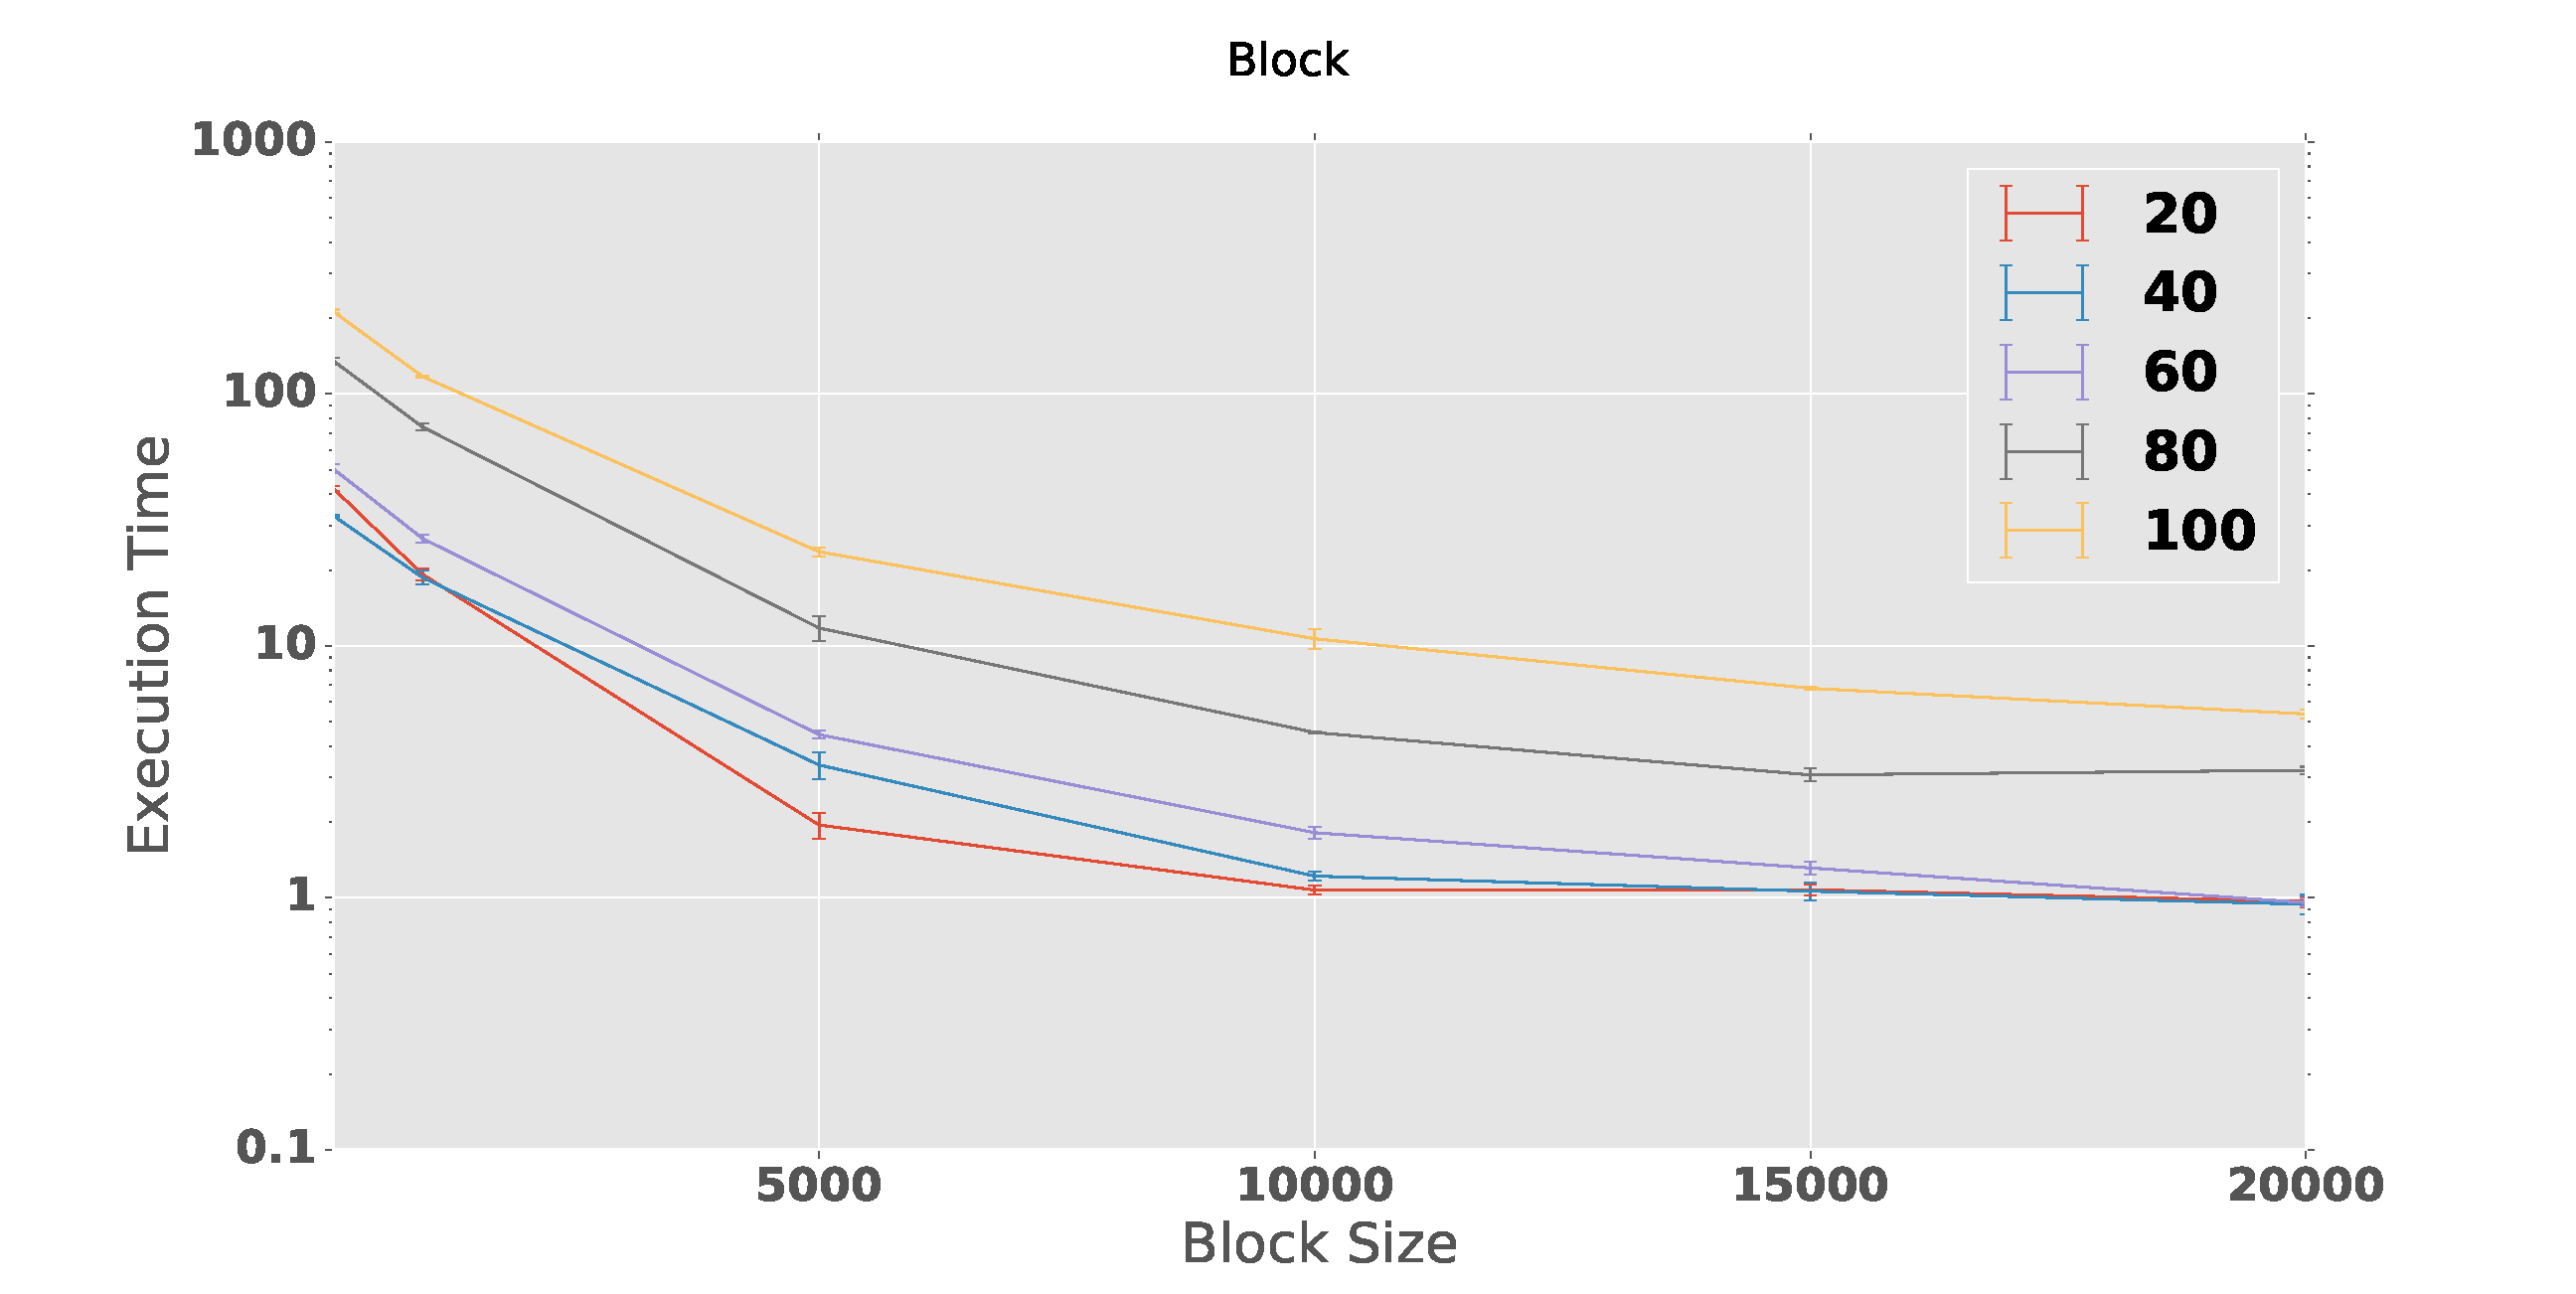
\includegraphics[width=0.95\textwidth]{figs/prefetch-block.eps}
	\caption{Average Execution time for A* search of different path lengths using a block prefetcher}
	\label{fig:prefetch-block}
\end{figure}
\begin{figure}[htbp]
	\centering
	\includegraphics[width=0.95\textwidth]{figs/prefetch-misses-block.eps}
	\caption{Graph miss rate for A* search of different path lengths using a block prefetcher}
	\label{fig:prefetch-miss-block}
\end{figure}
\begin{figure}[htbp]
	\centering
	\includegraphics[width=0.95\textwidth]{figs/prefetch-dbcost-block.eps}
	\caption{Average cost of store miss for A* search of different path lengths using a block prefetcher}
	\label{fig:prefetch-dbcost-block}
\end{figure}

Finally, we examine the effects on performance of using the \textit{block}
prefetcher (Figure~\ref{fig:prefetch-block}). Predictably, the overall
execution time of A* reduces as the block size increases. This happens because
the average cost of a graph miss remains roughly constant as block size
increases (Figure~\ref{fig:prefetch-dbcost-block}), but more vertices are
added to the graph store each time. This reduces the graph miss rate
(Figure~\ref{fig:prefetch-miss-block}), which causes a corresponding decrease in execution
time. However, I found that this reduction slows after a block size of around
15000, with an  overall execution time of between one and ten seconds. Since
both lookahead prefetchers achieved significantly shorter execution times of around 0.1s, and the
rate of improvement for the block prefetcher had stalled, no further
experiments were run at larger block sizes. 

It is interesting that this result contradicts the earlier one from Yoneki et
al., who found that the block prefetcher offered better performance than a
lookahead approach. Since we cannot make absolute comparisons between my test
platform and theirs, we can only speculate about the cause of this disparity.
It may be the case that my block prefetcher runs more slowly, which could be
caused by my using a larger dataset (although the same DIMACS dataset is cited
in the original Crackle report, several sizes are available and this detail is
not reported). It is also possible that improvements to PostgreSQL since 2012
have made the index lookups in this dataset perform more quickly, or that
indexes were misconfigured in the edge relation for the Crackle tests. These
indexes are critical to achieving good lookahead performance, and indeed
without them a block prefetcher performs significantly better on my setup.


For subsequent experiments, I used a CTE lookahead prefetcher with lookahead depth
5, since this offered a reliably good performance across all path lengths. 


\section{Query Performance} % (fold)
\label{sec:query_performance}
 
Having established an appropriate prefetching strategy, the next task is to
verify the hypothesis motivating Grapht's development: that there exists a significant
performance difference between PostgreSQL and Neo4J for certain queries.
Informally, we expect Neo4J to perform better for ``graph-centric'' queries,
whereas we expect PostgreSQL to perform better for ``row-centric'' queries. A
graph-centric query will tend to have the following features:

\begin{itemize}
	\item The absence or existence of edges between vertices is of greater interest than the attributes of the edges or vertices
	\item Only a local part of the graph need be considered to satisfy the query
\end{itemize}

In contrast, a row-centric query will place equal weight on the
attributes of entities as on the topology of the graph, and will typically
need to consider vertices and edges which are not necessarily connected to one
another. 

Specific queries were chosen as representative of each of these categories,
motivated by the mapping problem described in Chapter~\ref{ch:introduction}.
To represent graph-centric queries, an A* search query was used. This
satisfies the requirements, since the presence or absence of edges is what
characterises a path between two points, and attributes of the vertices are
otherwise ignored. Additionally, a solution can be found by searching through
only vertices local to the start point, rather than needing to look at the entire
graph. To represent row-centric queries, a string-matching query was chosen,
which identifies the vertex with a payload which most closely matches some user-specified string. A match is determined using by calculating the Levenshtein
distances\footnote{Informally, the Levenshtein distance is the minimum number
of single-character edits required to change one word into another} between
the two strings.  This is close to the kind of  query required to find a
location by name based on an approximate string search in a mapping application, and
is clearly row-centric since the vertex payload is of main interest, and
every vertex in the graph must be considered in case it has the closest match.


\subsection{Performance of Graph-centric Queries} % (fold)
\label{sub:performance_of_graph_centric_queries}

To generate random queries for the A* search, a similar methodology was
employed as for the prefetcher queries described in
Section~\ref{sec:prefetcher_performance}.  Paths were chosen to be of specific
lengths of 20, 40, 60, 80 or 100 hops, so that the average solution time would not
be dominated by the execution time required to find particularly long paths.
Degenerate cases are still possible with a fixed number of hops, however,
as the heuristic guiding A* may lead the search in a suboptimal direction. To 
minimise the impact of this, twenty routes for each path length were examined,
and the average time for all routes is presented here.

Finally, variation in performance might be due to differences in three
implementations of A*. To avoid this, a single Scala implementation was prepared, with three
adaptors responsible for fetching data from the relevant stores. For Neo4J and
Grapht, the direct API was used rather than the declarative interface.
Although it is possible to create an implementation of the A* algorithm
entirely in SQL, the lack of an efficient way to create a priority queue makes
performance unfairly low. Similarly, the Neo4J API provides a direct
\texttt{astar} method which performs the full computation internally, but it
would be unfair to compare its performance against another system which needs
to transfer data from store to external application at each iteration, since
Neo4J here does not suffer from the transfer latency. By providing a single A*
implementation for all three databases, we narrow the focus of our test to look solely at 
evaluating their performance as a data store, rather than as an algorithm implementation
platform.

\begin{figure}[htbp]
	\centering
	\includegraphics[width=0.95\textwidth]{figs/astargraph.eps}
	\caption{Average A* Execution time for paths of varying length across three database engines}
	\label{fig:astargraph}
\end{figure}

Figure~\ref{fig:astargraph} shows the average time taken to find each path.
 We
first notice that using Neo4J does indeed allow us to find a path significantly faster
than PostgreSQL -- a difference of nearly 1000x across all path lengths. This is
unsurprising since A* is an archetypal example of a very local, topology-focussed algorithm, around which we expect a graph-centric database like Neo4J to
be optimised. 

As hoped, Grapht bridges the performance gap between the two systems. Although
Neo4J's optimisations still grant it a performance advantage of around 35x,
Grapht completes search queries almost 30x faster than PostgreSQL on average. 
This is a particularly pleasing result given that this performance improvement 
has been given ``for free:'' no changes have been made to the source data at all.
By simply redirecting queries to pass through Grapht instead of
directly to PostgreSQL, A* performance can be significantly improved.

% subsection performance_of_graph_centric_queries (end)

\subsection{Performance of Row-Centric Queries} % (fold)
\label{sub:performance_of_row_centric_queries}

\begin{figure}[htbp]
	\centering
	\includegraphics[width=0.95\textwidth]{figs/levengraph.eps}
	\caption{Average Levenshtein-search execution time for 100 queries across three database engines}
	\label{fig:levengraph}
\end{figure}

To generate Levenshtein distance queries, a random number was generated, and
an MD5 string was created from it. This string  was used as the user-supplied
search string. Figure~\ref{fig:levengraph} shows the time taken for each of
the database systems to identify the vertex with the smallest Levenshtein
distance from the user-supplied string. Here, we see the opposite results to
the A* query. PostgreSQL completes the query significantly faster than Neo4J,
by about 6x. This is not such a large performance gap as the 1000x seen in the
previous subsection, and it seems likely that the cost of the query is largely
dominated by the cost of calculating the Levenshtein distances. This cost will
be comparable for the two engines, with the performance difference instead coming
from PostgreSQL's row-centric optimisations.

Since Grapht builds on top of a standard relational database, it is able to
simply forward the query on to PostgreSQL and achieve exactly the same
performance. By doing this, we have improved significantly on Neo4J's worst-case
performance.

% subsection performance_of_row_centric_queries (end)

\subsection{Performance of Hybrid Queries} % (fold)
\label{sub:performance_of_hybrid_queries}

Finally, we wish to consider not simply the performance of graph and row-centric queries in isolation, but also their performance when they are combined as in our
motivating example. To create this kind of query, we use first a Levenshtein
distance query to select a target vertex, and then perform an A* search from
some pre-selected source vertex (as if our user was searching for a route to
some destination by name). An appropriate source vertex was selected before
tests were run in order to ensure that the shortest paths were of a comparable
length.
% TODO: again group by path length?

\begin{figure}[htbp]
	\centering
	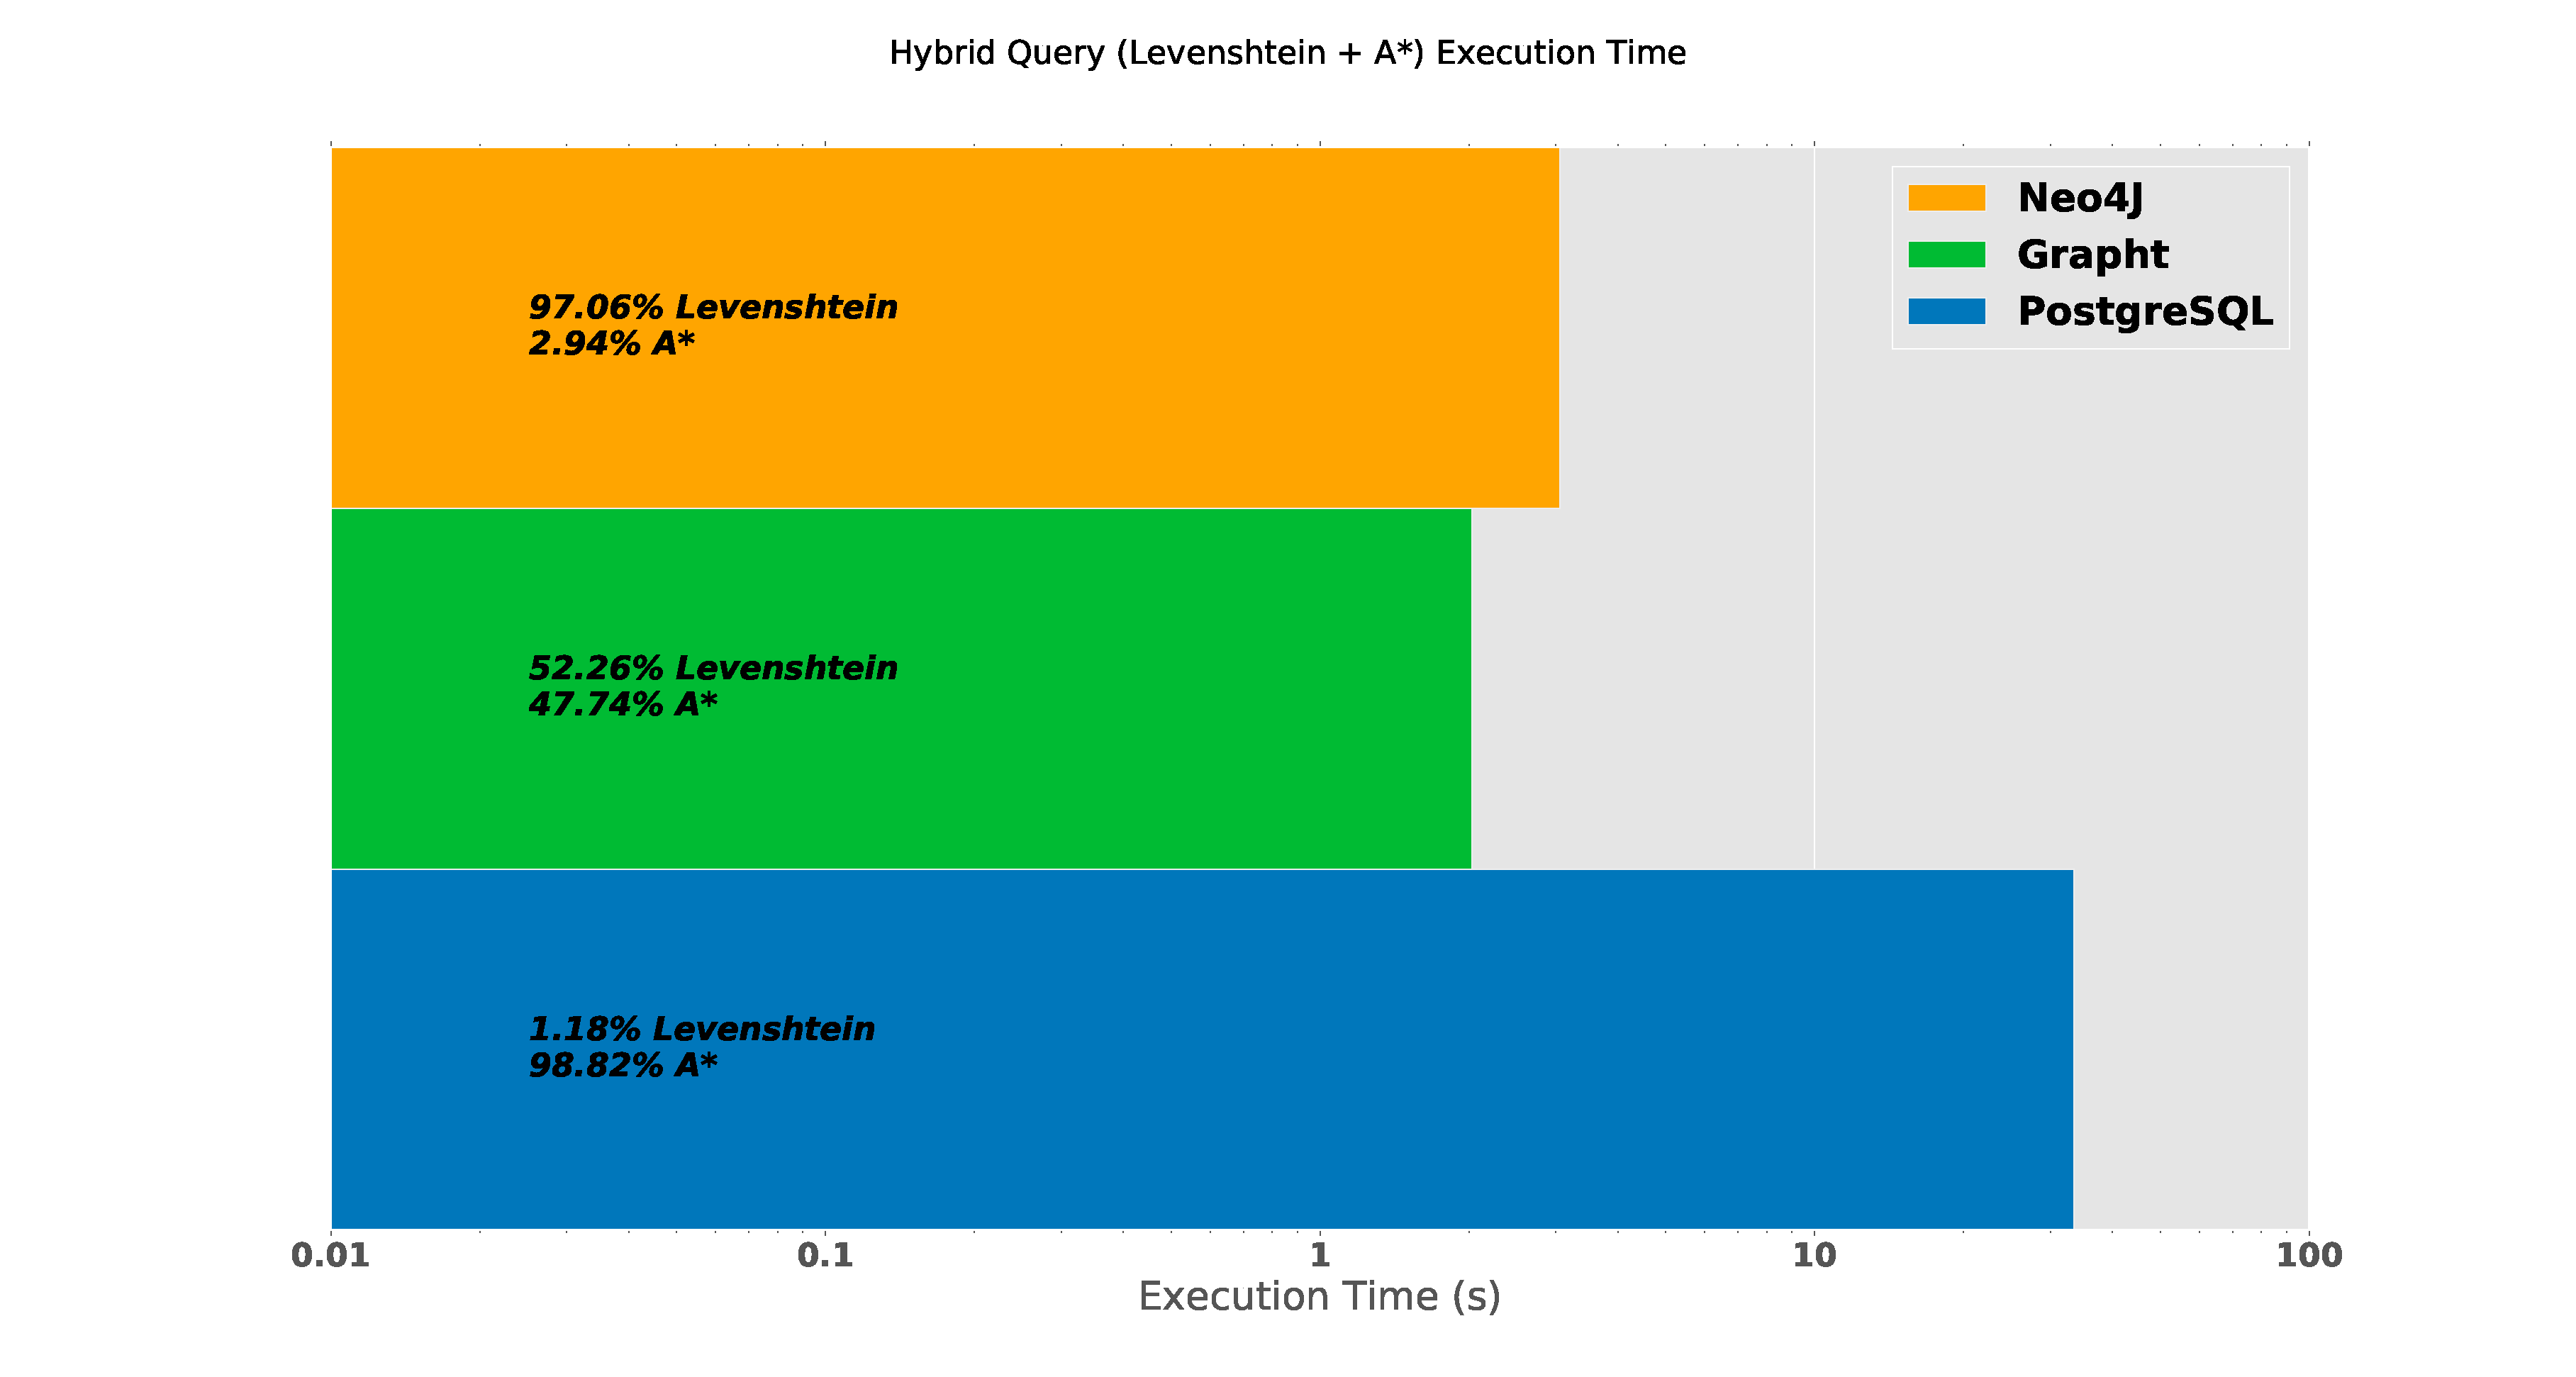
\includegraphics[width=0.95\textwidth]{figs/hybridgraph.eps}
	\caption{Average Execution time for 100 queries consisting of a minimum Levenshtein-distance search and an A* path search across three database engines. The percentage of time
	spent performing each of the two parts of the query is annotated for each engine.}
	\label{fig:hybridgraph}
\end{figure}

Figure~\ref{fig:hybridgraph} shows the average execution time for these hybrid
queries. In this scenario, Neo4J once again maintains a lead over PostgreSQL,
thanks to it's 1000x performance difference for the A* component of the search. More interesting, however,
is the fact that Grapht, by improving upon the worst-case performances of both
other systems, has managed to outperform both commercial systems. 

In reality, it would be impossible to select a database system based on these
benchmarks, without first determining exactly the type of queries which will
most often be encountered in production. If a workload is identified which is
dominated by graph-centric queries, it is likely that Neo4J would be the best
choice, as it will not suffer enough from occasional row-centric queries to
outweigh the benefits of the graph-centric optimisations. For workloads which
are evenly balanced between graph and row-centric queries however, a hybrid
system is able to outperform both specialised alternatives. Indeed, even if
the workload is mostly row-centric, it may wise to choose Grapht over
PostgreSQL alone, since there is no performance loss for row-centric queries,
and gains are possible for occasional graph-centric queries. This suggests
that maintaining an in-memory graph layer may be a worthwhile improvement to
make more closely within PostgreSQL in future, rather than needing to exist as
an optional add-on.



% subsection performance_of_hybrid_queries (end)
% section query_performance (end)


\section{Usability of Query Systems} % (fold)
\label{sec:usability_of_query_systems}

% TODO: These paragraphs are in a funny order!

In the previous section, I performed a quantitative analysis of the
performance of three database systems for graph-centric, row-centric and
hybrid queries. Performance is only one aspect contributing to the
success of  a system, however. Cost of deployment, or ease of use during development are other crucial
factors. If new custom queries are written frequently or on an ad-hoc basis, then
slow-running but quick-to-write queries may obtain an answer to an information need
more quickly overall.  

There are five interfaces to consider in this evaluation. Neo4J offers two
interfaces: a lightweight declarative query language called \textit{Cypher},
and a Java API more appropriate for complex graph
algorithms. PostgreSQL only offers one interface through SQL. Finally, Grapht
takes the same approach as Neo4J in offering both a programmatic API and a
declarative query language based on SQL called \textit{gSQL}.


When considering the cost of deployment of a new database system, the time
taken to learn to use the new system should also be examined. It is clearly
desirable from an ease-of-learning perspective to only need a single
interface. Introducing a second interface is likely to create confusion about
which one to use in different contexts, and at the very least increases the
amount of learning required to effectively use the system to its full
potential. One might first explore why it is that PostgreSQL can afford to
take provide a single interface, while the more graph-oriented approaches must
provide a lower-level API alongside a declarative query language. The answer
lies in considering the relative search spaces of the two problems. Various
optimisations and heuristics are possible to reduce the cost of traversing a
tabular relation, but in the worst case it is always possible to retrieve a
result in linear time by simply enumerating each row. The same is not true
when considering paths through a graph. The number of possible paths grows
exponentially with each additional hop in the path, meaning that for most
problems it is not practical to simply enumerate all possible paths when
searching for a single one. Instead, an intelligent approach is required to
direct traversal through the graph.

Cypher, having been in development for some time, has the ability to exploit
certain statistics and heuristics in order to slightly cut down the search
space, but does not avoid the problem in any real way. To find the shortest
path between two points using Cypher, for example, one must still enumerate all
possible paths between the points, and rank them by increasing length. To
avoid this, a large number of built-in functions are provided (such as
\texttt{shortestpath}, which can be used to avoid this particular situation). However these built-in
functions do not truly address the shortcoming of the language, which cannot
be used to express custom traversal strategies through large graphs. 
When using Grapht's or Neo4j's traversal API directly, the user
implements their own traversal strategy, removing the guesswork required for a
declarative interface. gSQL sacrifices some of the declarative nature of the
query language by allowing users to specify a traversal strategy with a
\texttt{TRAVERSE BY} clause. This allows solutions to be found for a query
more quickly, though at the cost of slightly more complicated query language.

A second factor limiting the expressiveness of a query language is the ability to create and manipulate data structures. Almost all
algorithms manipulate as part of their operation some central data
structure. It is often difficult to define these structures using  a
declarative query language, which typically tries to abstract away from this kind of
implementation detail.
With some creativity, it is often possible to manage a workaround in SQL, by
using temporary tables to encode the data structures required. A priority
queue can be implemented in this way (as required for a full-SQL
implementation of A*), though it will rarely perform as well as a solution
using binary heaps. This is not possible at all in Cypher, which can perform
little  more than pattern-matching on paths through the graph. The path
searches possible through gSQL are directed using the \texttt{TRAVERSE BY}
clause, which internally uses a priority queue to select upcoming expansions.
Much as it is possible to implement other data structures using a SQL table,
it is also possible to make creative use of Grapht's priority queue to
implement some other structures. For example, a ``last-in, first-out'' stack
can be created by using the insertion index as priority. This is not quite so
flexible as SQL, but again allows slightly more complicated algorithms to be
implemented entirely in gSQL than are possible in a language like Cypher.

Although some queries are totally inexpressible in a particular query
language, the ease of development for expressible queries should also be
considered. It is difficult to fully comment on the ease of use of the
different query languages without a formal usability study. However I would
expect to find that neither the Grapht nor Neo4J APIs would score highly in
this kind of study. Although these can be used to express any conceivable
query using the full power of any JVM language, needing to prepare and compile
code in order to express a simple query can be a is a huge complication,
especially when much of the code will be concerned with routine tasks like
establishing a database connection or deserialising data. Although Java is a
very well-known programming language, using APIs in this way also requires
that users be familiar with Java as well as the database API itself. For
newcomers, this means overcoming two learning barriers rather than just one.
Instead, I would expect that Cypher obtain a high usability score for novices,
since its pattern-matching queries are expressed in a fairly intuitive visual
language. On the other hand, SQL is much  more likely to have been encountered
before by experienced developers, which would presumably lead to a higher
score for this audience. gSQL, as a relatively small extension on top of SQL, would likely be
found easier to use by experienced developers than by novices.


% subsection expressiveness_of_query_systems (end)
% When considering the cost of deployment of a new database system, the time
% taken to learn to use the new system should also be examined. If the data originally
% comes from a relational data source (as most production data sources are), this
% cost of transition is one area in which Grapht particularly shines. In this situation, no
% changes to the underlying RDBMS need be made, and since the gSQL query
% language is a relatively small extension to standard SQL, there is only a small learning barrier.

